\section{Gleitobjekte (floats)}
Im Normalfall werden Objekte nicht genau dort im Text platziert, wo sie inhaltlich auch hingehören. \LaTeX{} versucht viele typographische Regeln zu erfüllen, um ein \enquote{korrektes} Schriftbild zu erreichen. Diese Regeln schaffen etwas Freiraum und erhöhen die Lesefreundlichkeit. Deshalb werden Tabellen und Abbildungen automatisch an die nächstmögliche geeignete Stelle \enquote{gleiten} und nachfolgende Objekte vor sich her schieben (quasi eine Warteschlange), bis das Dokument zu ende ist oder der Befehl \verb|\clearpage| eingegeben wird.

Um so eine Gleitumgebung zu schaffen stellt \LaTeX{} die beiden Umgebungen \texttt{figure} und \texttt{table} zur Verfügung. Bei Blocksatz ist es also so, dass Bilder und Tabellen am oberen oder unteren Blattrand, oder auf einer eigenständigen Seite (ohne Text) platziert werden. Dies, weil der Float-Specifier ohne Angabe auf \texttt{[tbp]} gesetzt ist (top, bottom, page). \textbf{Dies sollte immer die erste Wahl sein.}

Hat man jedoch sehr viele Bilder oder ist mit den automatisch gesetzten Bildpositionen nicht einverstanden, so ist eine Nachbearbeitung ganz am Schluss sinnvoll.
Durch Setzen von \texttt{[t]} oder \texttt{[b]} kann nach Belieben eingegriffen werden.
Sollte das immer noch nicht reichen können durch ein zusätzliches \texttt{!} (bang) die \LaTeX-Regeln für den Mindestanteil an normalem Text pro Seite umgangen werden.

\subsection{Abbildungen (figure)}
Eine Abbildung beginnt mit \verb|\begin{figure}| und endet mit \verb|\end{figure}|.
Dazwischen stehen Anweisungen für das Hinzufügen der Grafik, der Bildunterschrift und des Labels für die Referenzierung. Oft wird der Parameter \texttt{size=faktor} verwendet. Dieser hat jedoch den Nachteil, dass er abhängig von der Originalgrösse der Grafik ist. Besser ist die Verwendung des Parameters \texttt{width}. Dazu folgendes Beispiel, welches der Abbildung~\ref{fig:Figure} entspricht:

\begin{verbatim}
\begin{figure}[b]
  \centering
  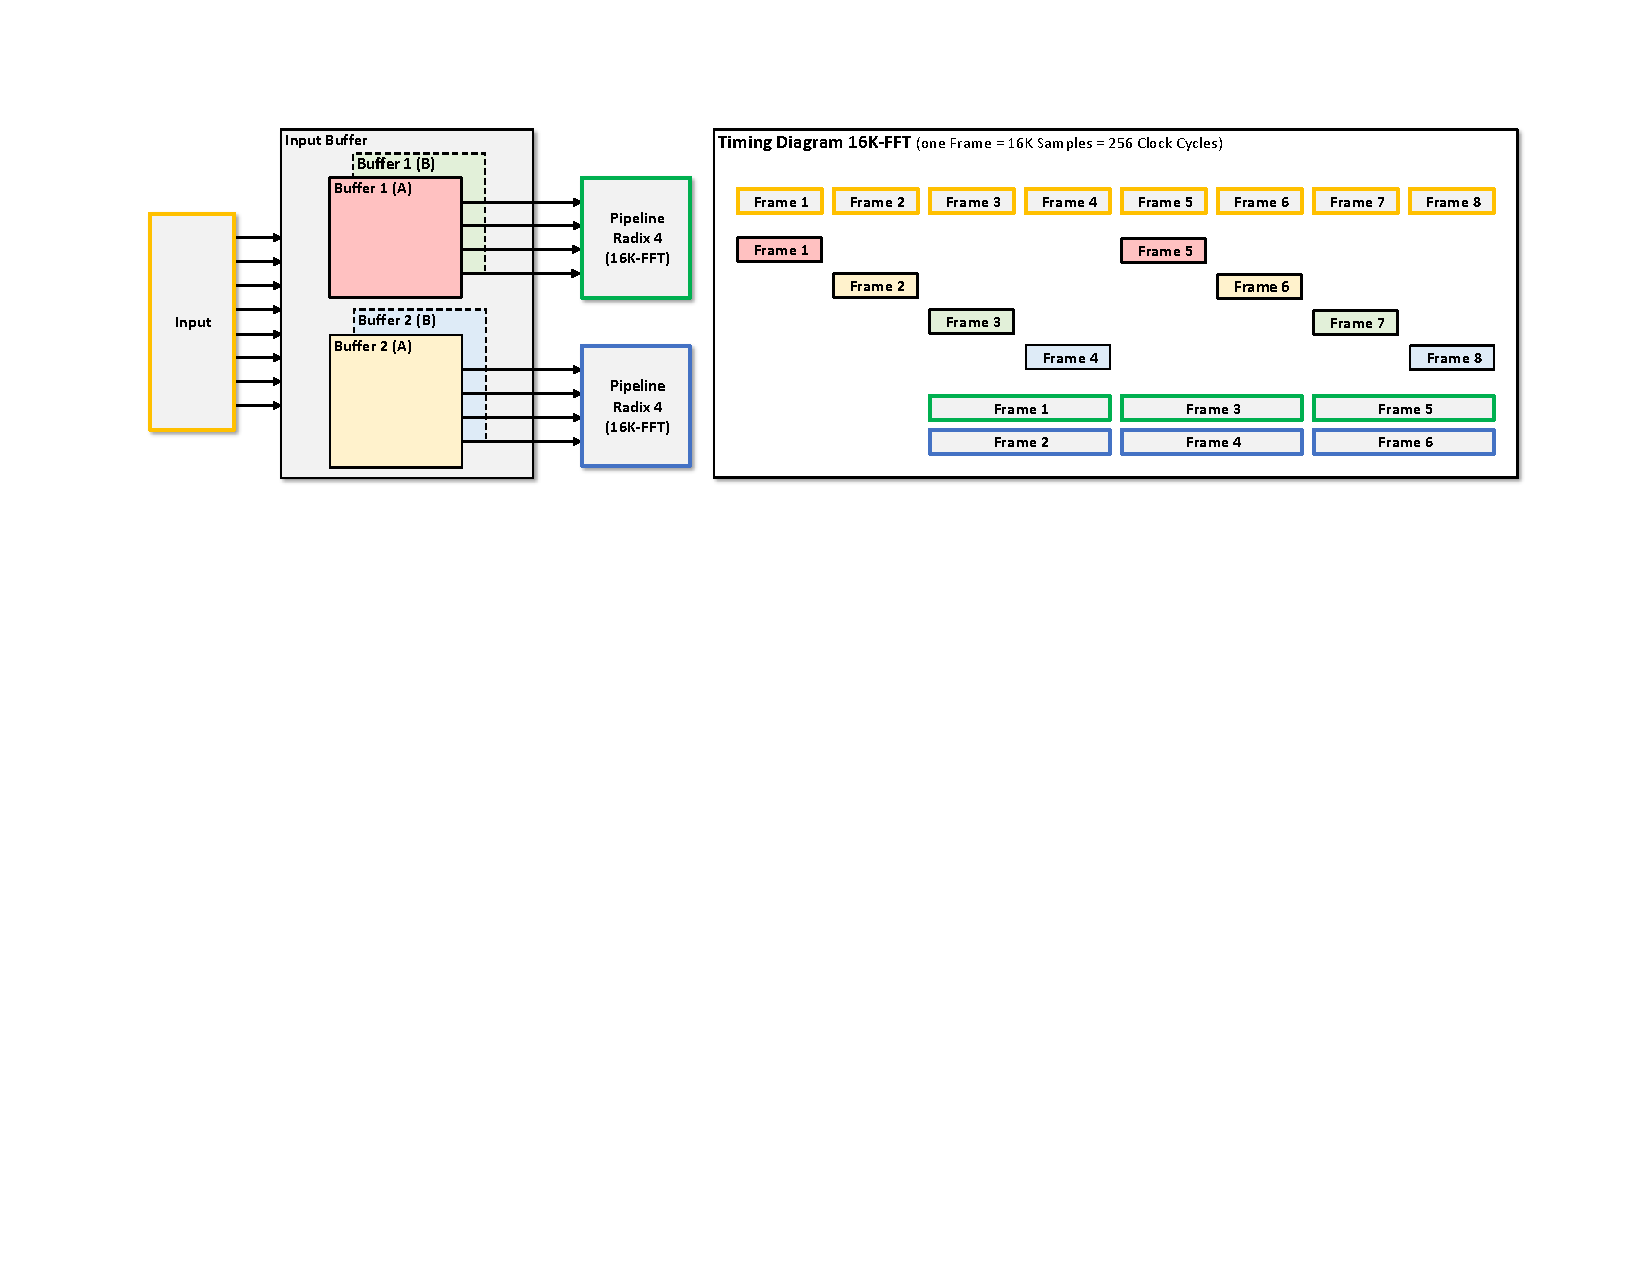
\includegraphics[width=0.9\linewidth]{beispiel.pdf}
  \caption{Dies ist ein Beispiel für eine Abbildung.}
  \label{fig:Figure}
\end{figure}
\end{verbatim}

\begin{figure}[b]
\centering
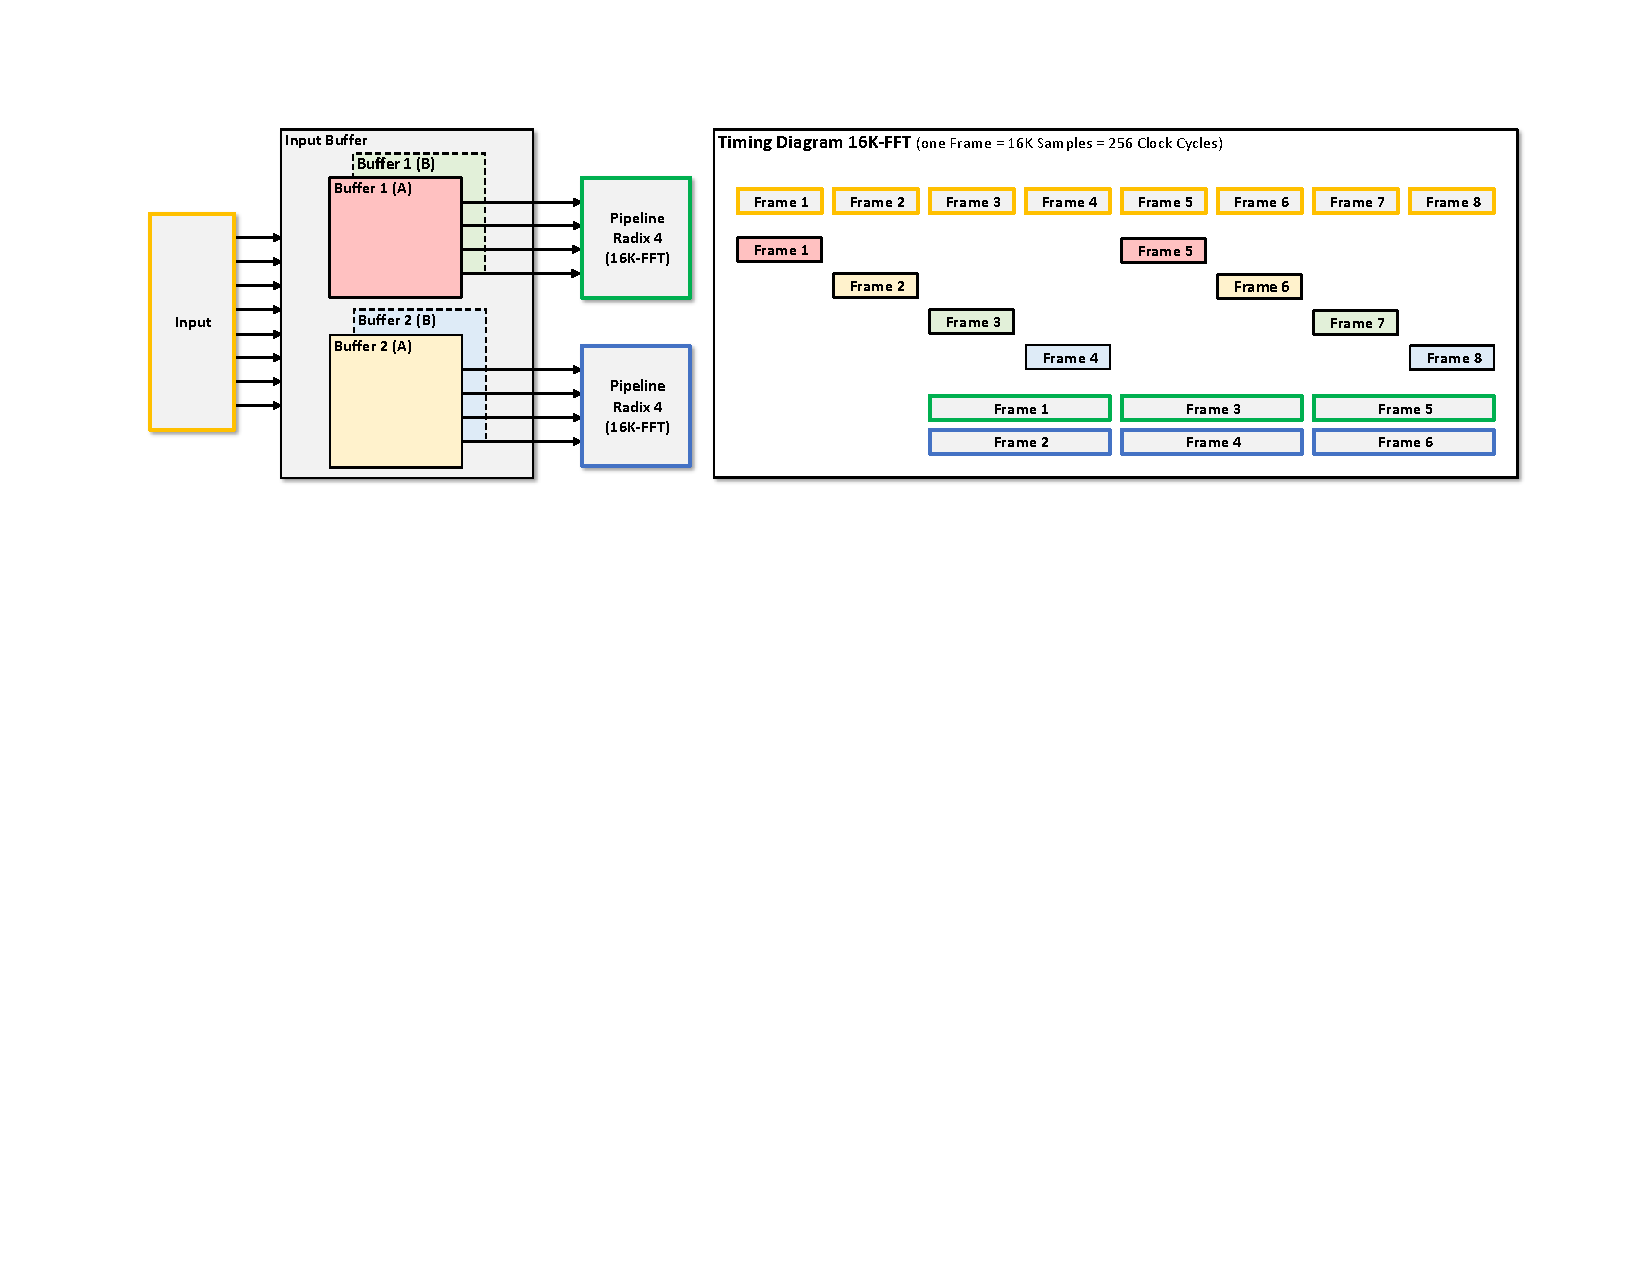
\includegraphics[width=0.9\linewidth]{beispiel.pdf}
\caption{Dies ist ein Beispiel für eine Abbildung.}
\label{fig:Figure}
\end{figure}

\subsubsection{Subfigures}
Hat man mehrere kleine Bilder (die irgendwie zusammengehören), kann man diese platzsparend in einer Subfigure anordnen. In Abbildung~\ref{fig:Subfigure} auf Seite~\pageref{fig:Subfigure} sieht man ein kleines Beispiel von Subfigures. Für diese wird das Package \verb|subfig| verwendet.

\begin{figure}[t]
\centering
\subfloat[Bild 1]{\rule{4cm}{3cm}}\qquad
\subfloat[Bild 2]{\rule{4cm}{3cm}}\qquad
\subfloat[Bild 3]{\rule{4cm}{3cm}}
\caption{Ein einfaches Beispiel für eine Abbildung mit mehreren Bildern.}
\label{fig:Subfigure}
\end{figure}

\subsection{Tabellen (table)}
Eine Tabellen beginnt mit \verb|\begin{table}| und endet mit \verb|\end{table}|.
Dazwischen stehen Anweisungen für das Erstellen der eigentlichen Tabellenanordnung, die Tabellenbeschreibung und ein Label für die Referenzierung. Dazu ein Beispiel, welches der Tabelle~\ref{tab:Table1} entspricht:

\begin{table}[b]
\centering
\begin{tabular}{C{1cm} C{2.5cm} C{2cm}|C{2cm} C{2.5cm} C{1cm}} 
\multicolumn{3}{c|}{\textbf{Normally Ordered Input}} & \multicolumn{3}{c}{\textbf{Digit-Reversed Output}} \\
{Index} & {Base 2} & {Base 4} & {Base 4} & {Base 2} & {Index} \\ \hline\hline 
60    &   11 11 00    & 330    & 033    & 00 11 11    &    15\\
61    &   11 11 01    & 331    & 133    & 01 11 11    &    31\\
62    &   11 11 10    & 332    & 233    & 10 11 11    &    47\\
63    &   11 11 11    & 333    & 333    & 11 11 11    &    63\\
\end{tabular}
\caption{Das erste Beispiel für eine Tabelle.}
\label{tab:Table1}
\end{table}

\begin{verbatim}
\begin{table}[b]
  \centering
  \begin{tabular}{C{1cm} C{2.5cm} C{2cm}|C{2cm} C{2.5cm} C{1cm}} 
  \multicolumn{3}{c|}{\textbf{Normally Ordered Input}}
    & \multicolumn{3}{c}{\textbf{Digit-Reversed Output}} \\
  {Index}& {Base 2} & {Base 4}& {Base 4} & {Base 2} & {Index}\\ \hline\hline 
    60   & 11 11 00 &   330   &   033    & 00 11 11 &   15   \\
    61   & 11 11 01 &   331   &   133    & 01 11 11 &   31   \\
    62   & 11 11 10 &   332   &   233    & 10 11 11 &   47   \\
    63   & 11 11 11 &   333   &   333    & 11 11 11 &   63   \\
  \end{tabular}
  \caption{Das erste Beispiel für eine Tabelle}\label{tab:DigitReverse}
\end{table}
\end{verbatim}

\textbf{Bei Tabellen gilt grundsätzlich: \enquote{Weniger ist manchmal mehr}. Somit sollte man auf möglichst viele durchgezogene Linien verzichten.} Vor allem die äussere Umrandung ist oft überflüssig. Nur wenn Linien dazu gedacht sind, Gruppen zu trennen oder zusammengehörige Blöcke zu kennzeichnen, dann sollen sie eingefügt werden.

Oft hat man im ersten Bericht keine Zeit für die saubere Gestaltung mit \LaTeX. Da bietet sich die Möglichkeit, Tabellen im Excel zu erstellen und diese als Bild mit \verb|\includegraphics{}| zwischen die \texttt{table}-Umgebung zu setzen.

Weiter gilt auch, dass sehr grosse Tabellen (z.\,B. Messprotokolle, Portmaps, \dots) im Anhang abgelegt werden können. Falls notwendig kann ein kleiner, aussagekräftiger Ausschnitt davon im Dokument eingefügt werden.

Tabellen, welche eine komplizierte Formatierung aufweisen (z.\,B. Projektpläne), können im Standalone-Modus in eine eigenständige Datei geschrieben werden und dann eingefügt werden oder man nimmt die vorhandene Excel-Tabelle und wandelt sie in ein PDF und fügt sie ebenfalls als ganze Seite dem Anhang hinzu.

Weitere Tabellen-Beispiele sind in Tab.~\ref{tab:TabelleComplex} gezeigt.

\begin{table}[b]
\centering
\begin{tabular}{>{\tt}C{2.3cm}| >{\tt}L{4cm}| L{7.2cm}} 
\normalfont\textbf{Parameter} & \normalfont\textbf{Structure} \small(row vector) & \textbf{Description} \\ \hline\hline 
\multirow{3}{*}{W}          & isSigned            & 1 = signed, 0 = unsigned    \\ \cline{2-3}
                            & WordLength          & Total word length of output (incl. sign bit)  \\ \cline{2-3} 
                            & FracLen             & Number of fractional bits     \\ \hline
\multirow{3}{*}[-0.5\baselineskip]{options}    & Scaling             & Number of decimal places to shift. For more information read the manual. \\ \cline{2-3}
                            & RoundingMethod      & 0 = Nearest, 1 = Ceiling, 2 = Convergent\\ \cline{2-3} 
                            & OverflowAction      & 0 = Saturate, 1 = Wrap     \\ \hline
\multirow{2}{*}{reporting}  & ShowOuputString    & Displays information to each conversation \\ \cline{2-3}
                            & CheckOverflow       & Enable the overflow check     \\ \hline
\end{tabular}

\vspace*{6ex}

\begin{tabular}{lllllllllllllllll}
  \hline
  Measures & Task &\multicolumn{4}{c}{Method 1} & & \multicolumn{4}{c}{Method 2} & &\multicolumn{4}{c}{Method 3} & p-value \\
  \hline
  && 1 & 2 & 3 & 4 & & 1 & 2 & 3 & 4 & & 1 & 2 & 3 & 4 & \\
  \cline{3-6} \cline{8-11} \cline{13-16}
  \multirow{3}{*}{Quality} & A \\
  & B \\
  & C \\
  \hline
  \multirow{3}{*}{Time} & A \\
  & B \\
  & C \\
  \hline
  \multirow{3}{*}{Cost} & A \\
  & B \\
  & C \\
  \hline
\end{tabular}
\caption{Beispiele mit komplizierter Zellenstruktur und automatischer Schrifteinstellung in zwei Kolonnen.}
\label{tab:TabelleComplex}
\end{table}
